\section{Problem Description}

First, some notation used in the rest of the paper.

Our goal is to take the user's complaints about the current state
of the database, and identify transformations over the database
query log that, when applied to the database, ``fixes'' these
complaints.  Although the general formulation of the problem that
we will introduce is intractable, we will reduce the scope of the
problem to a useful and tractable version.  To begin, we will
introduce the notation that is used in the rest of the paper.

\stitle{Def 1 (Database, State, Query)}: Let a database
be defined as the result of applying a sequence of queries in the query log
$Q_{seq}=\{Q_1,..., Q_n\}$ to an initial database $D_0$.  
Applying the query log to the initial database 
results in $n$ intermediate database states $\{D_i = Q_i(D_{i-1}) | i \in [1, n]\}$.  
where $D_n = Q_{seq}(D_0) = Q_n(\ldots Q_1(D_0))$ is the current state of the database. 
We assume that a subset of the query log has been replaced with {\it corrupted queries} 
such that $D_n$ and $Q_{seq}$ differ from the true database state $D^*_n$ and query log $Q^*_{seq}$.

In our current problem, we only deal with non aggregation and non-join queries.
In addition, for ease of exposition, we assume that the database contains a single table $T$ 
($T^*$ in the true database) containing $m$ numerical attributes $a_1,\ldots,a_m$, 
where the primary key is $a_1$.  
In Section~\ref{blah}, we will describe how our techniques extend to multi-table databases.
\xxx{Define the scope of queries supported}



\stitle{Def 2 (Complaints and Complaint Sets)}:
The tuple-wise difference between two databases $D_1$ and $D_2$ can be viewed as a patch
$P_{D_1, D_2}$ that contains {\it difference pairs} $(t_i \in T, t^*_i \in T^*)$.
Similar to source code patches, patches can be applied to a database $P(D_n) = D^*_n$.
Each pair in a patch describes one of three error types that can be present in $D_n$:

\begin{itemize}
\item {\it ADD}: $t^*_i$ should be added to the database $(\textrm{null}, t^*_i)$
\item {\it DELETE}: $t_i$ should be removed from the database $(t_i, \textrm{null})$
\item {\it WRONG}: $t_i$ should be modified into $t^*_i$
\end{itemize}


The user provides a {\it complaint set} $C$ that specify the perceived incorrect tuples in $D_n$.
$C$ is simply a patch.
We define a complete complaint set when $C = P_{D_n, D^*_n}$.
In contrast, an {\it incomplete complaint set}  may contain complaints that are false negatives (insertions that should be in $C$ but are not),
false positives (deletions that are not present), and errors (proposed value of a $t'$ is incorrect).

The accuracy of an incomplete complaint set can be measured by the ratio $acc_C = \frac{|C \cap \Delta|}{|\Delta|}$.



\begin{figure}[h]
\centering
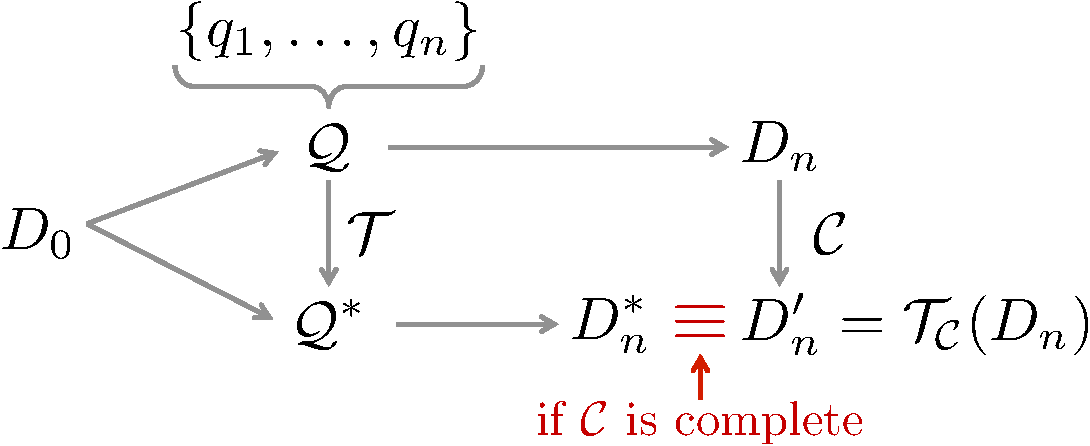
\includegraphics[width = 2in]{figures/probtransform}
\caption{Graphical depiction of the general XXX problem.}
\label{f:probtransform} 
\end{figure}



\subsection{Naive Formulation}

The most general version of the problem
(depicted in Figure~\ref{f:probtransform}) is to find a sequence of
transformations $T$ that insert, delete, and/or modify queries in $Q_{seq}$ 
such that the resulting sequence, $Q^'_{seq} = T(Q_{seq})$, resolves the user's complaint set. 

However this problem is ill-defined because there exist an unbounded set of transformations that
can resolve the user's complaint set.  A naive solution is to append to the query log a statement
that deletes all the records in the database, followed by a query that insert all of the correct records.
Unfortunately this naive solution does not help explain the complaints in any way!

\subsection{Constraints}

For this reason, we constrain the set of possible transformations $\mathcal{T}$ to the following:

\begin{itemize}
\item delete query
\item modify insert statement constants
\item modify constants in WHERE clause
\end{itemize}

Our transformations don't include adding new queries, synthesizing arbitrary queries, or modifying the
number of clauses in a WHERE condition.  We apply these restrictions because we believe it is more likely
for the user to mis-type a constant value as opposed to having an error in the query structure.

Futhermore we define a distance metric between two query logs in order to evaluate
the qulatiy of a transformation.
\xxx{define $\mathcal{T}$ here.}



\subsection{Problem Statements}

In this paper, we present three variants of this problem.

\begin{problem}[Prob-Complete]\label{prob:complete}
Given $C = P_{D_n, D^*_n}$, $Q_{seq}$, and the sequence of database states $D_0,\ldots,D_n$, 
identify a sequence of transformations $T$ such that:
\begin{CompactItemize}
\item $T(Q_{seq})(D_0) = C(D_n)$
\item $|T| = 1$
\item $T$ metric is minimized
\end{CompactItemize}
\end{problem}

This variation of the problme relaxes the constraint that the complaint set must be complete, and allows
for both false positives as well as false negatives.  The goal is the same, however the constraints are relaxed:

\begin{problem}[Prob-Incomplete]\label{prob:incomplete}
Given $C$ where $acc_C < 1$, $Q_{seq}$, and the sequence of database states $D_0,\ldots,D_n$, 
identify a sequence of transformations $T$ such that:
\begin{CompactItemize}
\item $T(Q_{seq})(D_0) = D^*_n$
\item $T$ metric is minimized.
\item $|T| = 1$
\end{CompactItemize}
\end{problem}

Finally, we extend the problem to allow transformations with one or more operations.

\begin{problem}[Prob-MultiQ]\label{prob:multi}
Given $C$ where $acc_C < 1$, $Q_{seq}$, and the sequence of database states $D_0,\ldots,D_n$, 
identify a sequence of transformations $T$ such that:
\begin{CompactItemize}
\item $T(Q_{seq})(D_0) = D^*_n$
\item $T$ metric is minimized.
\end{CompactItemize}
\end{problem}




\subsection{A Naive Approach}

\begin{itemize}
\item roll back complaints to penultimate state using algebraic expressions 
\item perturb each expression in query until the query result matches correct state
\item if an expression cannot be found, iterate
\end{itemize}


Not clear how to roll back complaints

Ways to perturb query expressions is unbounded

